\documentclass{beamer}
\usepackage[utf8]{inputenc}

\usetheme{Madrid}
\usecolortheme{default}
\usepackage{amsmath,amssymb,amsfonts,amsthm}
\usepackage{txfonts}
\usepackage{tkz-euclide}
\usepackage{listings}
\usepackage{adjustbox}
\usepackage{array}
\usepackage{tabularx}
\usepackage{gvv}
\usepackage{lmodern}
\usepackage{circuitikz}
\usepackage{tikz}
\usepackage{graphicx}
\usepackage{multicol}

\setbeamertemplate{page number in head/foot}[totalframenumber]

\usepackage{tcolorbox}
\tcbuselibrary{minted,breakable,xparse,skins}



\definecolor{bg}{gray}{0.95}
\DeclareTCBListing{mintedbox}{O{}m!O{}}{%
  breakable=true,
  listing engine=minted,
  listing only,
  minted language=#2,
  minted style=default,
  minted options={%
    linenos,
    gobble=0,
    breaklines=true,
    breakafter=,,
    fontsize=\small,
    numbersep=8pt,
    #1},
  boxsep=0pt,
  left skip=0pt,
  right skip=0pt,
  left=25pt,
  right=0pt,
  top=3pt,
  bottom=3pt,
  arc=5pt,
  leftrule=0pt,
  rightrule=0pt,
  bottomrule=2pt,
  toprule=2pt,
  colback=bg,
  colframe=orange!70,
  enhanced,
  overlay={%
    \begin{tcbclipinterior}
    \fill[orange!20!white] (frame.south west) rectangle ([xshift=20pt]frame.north west);
    \end{tcbclipinterior}},
  #3,
}
\lstset{
    language=C,
    basicstyle=\ttfamily\small,
    keywordstyle=\color{blue},
    stringstyle=\color{orange},
    commentstyle=\color{green!60!black},
    numbers=left,
    numberstyle=\tiny\color{gray},
    breaklines=true,
    showstringspaces=false,
}
%------------------------------------------------------------
%This block of code defines the information to appear in the
%Title page
\title %optional
{4.11.7}
\date{September 29,2025}


\author 
{Jnanesh Sathisha karmar - EE25BTECH11029}



\begin{document}



\frame{\titlepage}
\begin{frame}{Question}Find the equation of the planes passing through the intersection of the planes $\vec{r}.\brak{3\hat{i}+6\hat{j}}+12=0$ and $\vec{r}.\brak{3\hat{i}-\hat{j}+4\hat{k}}=0$ are at a unit distance from the origin.


\end{frame}



\begin{frame}{Equation}
Given details\\Plane 1:
\begin{align}
   \vec{r}.\brak{3\hat{i}+6\hat{j}}+12=0\\
   \myvec{3&6&0}\vec{r}+12=0\\
   \text{dividing the equation with 3:}\\
   \myvec{1&2&0}\vec{r}+4=0\\
   \Rightarrow \vec{n}_1^{\top}\vec{r}+d_1=0\\
   \text{Therefore :      }\\ \vec{n_1}^{\top}=\myvec{1 & 2 &0} \text{and}\  d_1=4
\end{align}
\end{frame}
\begin{frame}{Equation}
Plane 2:
\begin{align}
    \vec{r}.\brak{3\hat{i}-\hat{j}+4\hat{k}}=0\\
    \myvec{3 & -1 & 4}\vec{r}+0=0\\
    \text{similarly:}\\
    \vec{n_2}^{\top}=\myvec{3 & -1 & 4} \text{and}\ d_2=0
\end{align}
\end{frame}
\begin{frame}{Theoretical Solution}
plane passing through the intersection of the two given planes can be represented as a linear combination of their equations.
\begin{align}
    \brak{\vec{n_1}^{\top}+d_1}+\lambda\brak{\vec{n_2}^{\top}+d_2}=0
\end{align}
Rearranging them:
\begin{align}
    \brak{\vec{n_1}^{\top}+\lambda\vec{n_2}^{\top}}+\brak{d_1+ \lambda d_2}=0
\end{align}
\end{frame}

\begin{frame}{Theoretical Solution}
Substituting the values we get:
\begin{align}
    \brak{\myvec{1 & 2 & 0} + \lambda\myvec{3 & -1 & 4}}+\brak{4+\lambda.0}=0\\
    \myvec{1+3\lambda&2-\lambda&4\lambda}\vec{r}+4=0
\end{align}
This is the general equation for any plane passing through the line of intersection. Let's call the new normal vector $\vec{n}^{\top}=\myvec{1+3\lambda&2-\lambda&4\lambda}$ and the constant $d=4$\\

\end{frame}
\begin{frame}{Theoretical Solution}
Since the plane is at a unit distance from the origin
\begin{align}
    1&=\frac{|d|}{\norm{\vec{n}}}\\
    1&=\frac{4}{\sqrt{\brak{1+3\lambda}^2+\brak{2-\lambda}^2+\brak{4\lambda}^2}}\\
    &26\lambda^2+2\lambda-11=0
\end{align}
On solving the equation we get:
\begin{align}
    \lambda = \frac{-2 \pm 2\sqrt{287}}{52} = \frac{-1 \pm \sqrt{287}}{26}
\end{align}
\end{frame}
\begin{frame}{Theoretical Solution}
This gives us two possible values for $\lambda$, which means there are two planes that satisfy the given conditions.\\
The final plane equations are:
\begin{align}
    \vec{r} \brak{\brak{23 + 3\sqrt{287}}\hat{i} + \brak{53 - \sqrt{287}}\hat{j} + \brak{4\sqrt{287} - 4}\hat{k}} + 104 = 0\\
    \vec{r}\brak{\brak{23 - 3\sqrt{287}}\hat{i} + \brak{53 + \sqrt{287}}\hat{j} - \brak{4 + 4\sqrt{287}}\hat{k}} + 104 = 0
\end{align}

    
\end{frame}





\begin{frame}[fragile]
    \frametitle{C Code (1) - Function to store the points }

    \begin{lstlisting}
#include <stdlib.h>
#include <math.h>

void free_points(float* points) {
    if (points != NULL) {
        free(points);
    }
}
float* generate_plane_1_points(float y_min, float y_max, float z_min, float z_max, int num_steps) {
    if (num_steps <= 1) {
        return NULL;
    }
    int total_points = num_steps * num_steps;
    float* points = (float*)malloc(total_points * 3 * sizeof(float));
    if (points == NULL) {
        return NULL;
    }


    \end{lstlisting}
\end{frame}
\begin{frame}[fragile]
    \frametitle{C Code (1) - Function to store the points }

    \begin{lstlisting}
    float y_step_size = (y_max - y_min) / (num_steps - 1);
    float z_step_size = (z_max - z_min) / (num_steps - 1);
    int index = 0;
    for (int i = 0; i < num_steps; i++) {
        float y = y_min + i * y_step_size;
        for (int j = 0; j < num_steps; j++) {
            float z = z_min + j * z_step_size;
            float x = -2.0f * y - 4.0f;
            points[index++] = x;
            points[index++] = y;
            points[index++] = z;
        }
    }
    return points;
}
float* generate_plane_2_points(float x_min, float x_max, float y_min, float y_max, int num_steps) {
    if (num_steps <= 1) {return NULL;}
    \end{lstlisting}
\end{frame}
\begin{frame}[fragile]
    \frametitle{C Code (1) - Function to store the points }

    \begin{lstlisting}
    int total_points = num_steps * num_steps;
    float* points = (float*)malloc(total_points * 3 * sizeof(float));
    if (points == NULL) {return NULL;}
    float x_step_size = (x_max - x_min) / (num_steps - 1);
    float y_step_size = (y_max - y_min) / (num_steps - 1);
    int index = 0;
    for (int i = 0; i < num_steps; i++) {
        float x = x_min + i * x_step_size;
        for (int j = 0; j < num_steps; j++) {
            float y = y_min + j * y_step_size;
            float z = (-3.0f * x + y) / 4.0f;
            points[index++] = x;
            points[index++] = y;
            points[index++] = z;
        }
    }
    return points;
}
    \end{lstlisting}
\end{frame}

\begin{frame}[fragile]
    \frametitle{C Code (1) - Function to store the points }

    \begin{lstlisting}
float* generate_plane_3_points(float x_min, float x_max, float y_min, float y_max, int num_steps) {
    if (num_steps <= 1) {
        return NULL;
    }

    int total_points = num_steps * num_steps;
    float* points = (float*)malloc(total_points * 3 * sizeof(float));
    if (points == NULL) {
        return NULL;
    }
    
    const float sqrt287 = sqrtf(287.0f);
    const float A = 23.0f + 3.0f * sqrt287;
    const float B = 53.0f - sqrt287;
    const float C = 4.0f * sqrt287 - 4.0f;
    const float D = 104.0f;


    \end{lstlisting}
\end{frame}
\begin{frame}[fragile]
    \frametitle{C Code (1) - Function to store the points }

    \begin{lstlisting}
    float x_step_size = (x_max - x_min) / (num_steps - 1);
    float y_step_size = (y_max - y_min) / (num_steps - 1);

    int index = 0;
    for (int i = 0; i < num_steps; i++) {
        float x = x_min + i * x_step_size;
        for (int j = 0; j < num_steps; j++) {
            float y = y_min + j * y_step_size;
            float z = (-A * x - B * y - D) / C;

            points[index++] = x;
            points[index++] = y;
            points[index++] = z;
        }
    }
    return points;
}
    \end{lstlisting}
\end{frame}
\begin{frame}[fragile]
    \frametitle{C Code (1) - Function to store the points }

    \begin{lstlisting}
float* generate_plane_4_points(float x_min, float x_max, float y_min, float y_max, int num_steps) {
    if (num_steps <= 1) {
        return NULL;
    }

    int total_points = num_steps * num_steps;
    float* points = (float*)malloc(total_points * 3 * sizeof(float));
    if (points == NULL) {
        return NULL;
    }

    const float sqrt287 = sqrtf(287.0f);
    const float A = 23.0f - 3.0f * sqrt287;
    const float B = 53.0f + sqrt287;
    const float C = -4.0f - 4.0f * sqrt287;
    const float D = 104.0f;


    \end{lstlisting}
\end{frame}
\begin{frame}[fragile]
    \frametitle{C Code (1) - Function to store the points }

    \begin{lstlisting}
    float x_step_size = (x_max - x_min) / (num_steps - 1);
    float y_step_size = (y_max - y_min) / (num_steps - 1);

    int index = 0;
    for (int i = 0; i < num_steps; i++) {
        float x = x_min + i * x_step_size;
        for (int j = 0; j < num_steps; j++) {
            float y = y_min + j * y_step_size;
            float z = (-A * x - B * y - D) / C;

            points[index++] = x;
            points[index++] = y;
            points[index++] = z;
        }
    }
    return points;
}
    \end{lstlisting}
\end{frame}
\begin{frame}[fragile]
    \frametitle{Python Code - Using Shared Object}
    \begin{lstlisting}
import ctypes
import numpy as np
import matplotlib.pyplot as plt
NUM_STEPS = 50
PLOT_RANGE = 10.0
plane_lib = ctypes.CDLL(./planes.so)

float_ptr = ctypes.POINTER(ctypes.c_float)

plane_lib.free_points.argtypes = [float_ptr]
plane_lib.free_points.restype = None
plane_lib.generate_plane_1_points.argtypes = [ctypes.c_float, ctypes.c_float, ctypes.c_float, ctypes.c_float, ctypes.c_int]
plane_lib.generate_plane_1_points.restype = float_ptr

plane_lib.generate_plane_2_points.argtypes = [ctypes.c_float, ctypes.c_float, ctypes.c_float, ctypes.c_float, ctypes.c_int]
plane_lib.generate_plane_2_points.restype = float_ptr
\end{lstlisting}
\end{frame}

\begin{frame}[fragile]
    \frametitle{Python Code - Using Shared Object}
    \begin{lstlisting}
plane_lib.generate_plane_3_points.argtypes = [ctypes.c_float, ctypes.c_float, ctypes.c_float, ctypes.c_float, ctypes.c_int]
plane_lib.generate_plane_3_points.restype = float_ptr

plane_lib.generate_plane_4_points.argtypes = [ctypes.c_float, ctypes.c_float, ctypes.c_float, ctypes.c_float, ctypes.c_int]
plane_lib.generate_plane_4_points.restype = float_ptr


def get_plane_data(c_function, *args):
    points_ptr = None
    points_data = None
    total_points = NUM_STEPS * NUM_STEPS
\end{lstlisting}
\end{frame}
\begin{frame}[fragile]
    \frametitle{Python Code - Using Shared Object}
    \begin{lstlisting}
    try:
        points_ptr = c_function(*args)
        if not points_ptr:
            raise MemoryError("C function failed to allocate memory or returned NULL.")
        points_np_view = np.ctypeslib.as_array(points_ptr, shape=(total_points * 3,))
        points_data = np.copy(points_np_view)
    finally:
        if points_ptr:
            plane_lib.free_points(points_ptr)
    return points_data
print("Generating points for all planes...")
plane1_data_flat = get_plane_data(
    plane_lib.generate_plane_1_points, 
    -PLOT_RANGE, PLOT_RANGE, -PLOT_RANGE, PLOT_RANGE, NUM_STEPS
)
\end{lstlisting}
\end{frame}
\begin{frame}[fragile]
    \frametitle{Python Code - Using Shared Object}
    \begin{lstlisting}
plane2_data_flat = get_plane_data(
    plane_lib.generate_plane_2_points,
    -PLOT_RANGE, PLOT_RANGE, -PLOT_RANGE, PLOT_RANGE, NUM_STEPS)
plane3_data_flat = get_plane_data(
    plane_lib.generate_plane_3_points,
    -PLOT_RANGE, PLOT_RANGE, -PLOT_RANGE, PLOT_RANGE, NUM_STEPS)
plane4_data_flat = get_plane_data(
    plane_lib.generate_plane_4_points,
    -PLOT_RANGE, PLOT_RANGE, -PLOT_RANGE, PLOT_RANGE, NUM_STEPS)
print(f"Generated {plane1_data_flat.shape[0] // 3} points per plane and freed C memory.")
def reshape_for_plot(flat_data):
    points = flat_data.reshape(NUM_STEPS * NUM_STEPS, 3)
    X = points[:, 0].reshape(NUM_STEPS, NUM_STEPS)
    Y = points[:, 1].reshape(NUM_STEPS, NUM_STEPS)
    Z = points[:, 2].reshape(NUM_STEPS, NUM_STEPS)
    return X, Y, Z

\end{lstlisting}
\end{frame}
\begin{frame}[fragile]
    \frametitle{Python Code - Using Shared Object}
    \begin{lstlisting}
X1, Y1, Z1 = reshape_for_plot(plane1_data_flat)
X2, Y2, Z2 = reshape_for_plot(plane2_data_flat)
X3, Y3, Z3 = reshape_for_plot(plane3_data_flat)
X4, Y4, Z4 = reshape_for_plot(plane4_data_flat)
print("Plotting the planes...")
fig = plt.figure(figsize=(12, 10))
ax = fig.add_subplot(projection='3d')
ax.plot_surface(X1, Y1, Z1, cmap='viridis', alpha=0.7)
ax.plot_surface(X2, Y2, Z2, cmap='plasma', alpha=0.7)
ax.plot_surface(X3, Y3, Z3, cmap='inferno', alpha=0.7)
ax.plot_surface(X4, Y4, Z4, cmap='magma', alpha=0.7)
ax.set_xlabel('X-axis')
ax.set_ylabel('Y-axis')
ax.set_zlabel('Z-axis')
ax.set_title('planes')
plt.savefig("./figs/planes.png")
subprocess.run(shlex.split('termux-open ../figs/planes.png'))
plt.show()

\end{lstlisting}
\end{frame}


\begin{frame}{Plot-Using Both C and Python}
    \centering
    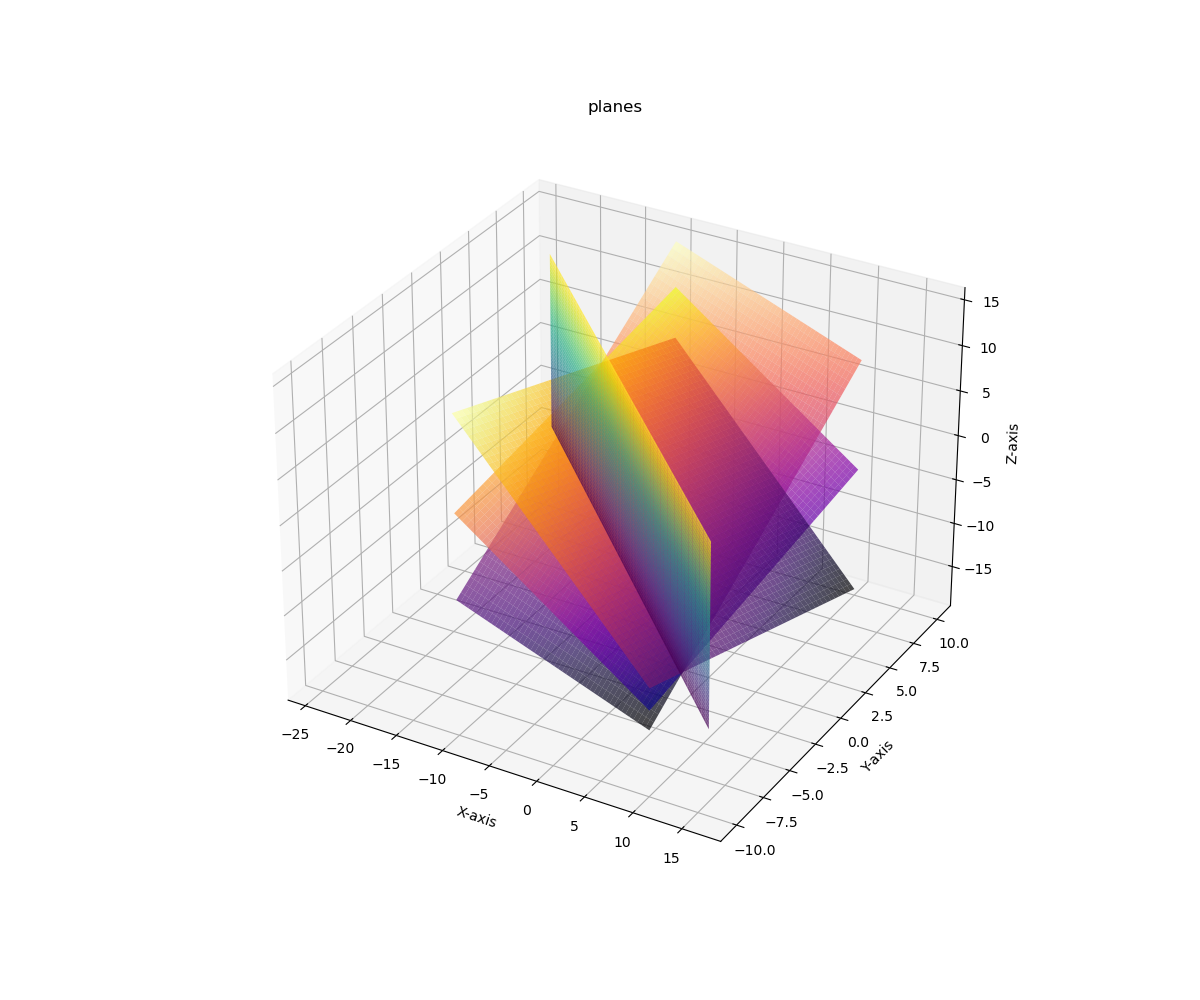
\includegraphics[width=\columnwidth, height=0.8\textheight, keepaspectratio]{figs/planes.png}     
\end{frame}

\begin{frame}[fragile]
    \frametitle{Python Code}
    \begin{lstlisting}
import numpy as np
import matplotlib.pyplot as plt
NUM_STEPS = 50
PLOT_RANGE = 10.0
def generate_plane_1_points_py(y_min, y_max, z_min, z_max, num_steps):
    y = np.linspace(y_min, y_max, num_steps)
    z = np.linspace(z_min, z_max, num_steps)
    Y, Z = np.meshgrid(y, z)
    X = -2.0 * Y - 4.0
    return X, Y, Z
def generate_plane_2_points_py(x_min, x_max, y_min, y_max, num_steps):
    x = np.linspace(x_min, x_max, num_steps)
    y = np.linspace(y_min, y_max, num_steps)
    X, Y = np.meshgrid(x, y)
    Z = (-3.0 * X + Y) / 4.0
    return X, Y, Z
\end{lstlisting}
\end{frame}
\begin{frame}[fragile]
    \frametitle{Python Code}
    \begin{lstlisting}
def generate_plane_3_points_py(x_min, x_max, y_min, y_max, num_steps):
    sqrt287 = np.sqrt(287.0)
    A = 23.0 + 3.0 * sqrt287
    B = 53.0 - sqrt287
    C = 4.0 * sqrt287 - 4.0
    D = 104.0  
    x = np.linspace(x_min, x_max, num_steps)
    y = np.linspace(y_min, y_max, num_steps)
    X, Y = np.meshgrid(x, y)
    Z = (-A * X - B * Y - D) / C
    return X, Y, Z
def generate_plane_4_points_py(x_min, x_max, y_min, y_max, num_steps):
    sqrt287 = np.sqrt(287.0)
    A = 23.0 - 3.0 * sqrt287
    B = 53.0 + sqrt287
    C = -4.0 - 4.0 * sqrt287
    D = 104.0
\end{lstlisting}
\end{frame}
\begin{frame}[fragile]
    \frametitle{Python Code}
    \begin{lstlisting}
    x = np.linspace(x_min, x_max, num_steps)
    y = np.linspace(y_min, y_max, num_steps)
    X, Y = np.meshgrid(x, y)
    Z = (-A * X - B * Y - D) / C
    return X, Y, Z
print("Generating points for all planes using Python...")

X1, Y1, Z1 = generate_plane_1_points_py(-PLOT_RANGE, PLOT_RANGE, -PLOT_RANGE, PLOT_RANGE, NUM_STEPS)
X2, Y2, Z2 = generate_plane_2_points_py(-PLOT_RANGE, PLOT_RANGE, -PLOT_RANGE, PLOT_RANGE, NUM_STEPS)
X3, Y3, Z3 = generate_plane_3_points_py(-PLOT_RANGE, PLOT_RANGE, -PLOT_RANGE, PLOT_RANGE, NUM_STEPS)
X4, Y4, Z4 = generate_plane_4_points_py(-PLOT_RANGE, PLOT_RANGE, -PLOT_RANGE, PLOT_RANGE, NUM_STEPS)

print(f"Generated points for {NUM_STEPS*NUM_STEPS} grid locations per plane.")
\end{lstlisting}
\end{frame}
\begin{frame}[fragile]
    \frametitle{Python Code}
    \begin{lstlisting}
print("Plotting the planes...")
fig = plt.figure(figsize=(12, 10))
ax = fig.add_subplot(projection='3d')

ax.plot_surface(X1, Y1, Z1, cmap='viridis', alpha=0.7)
ax.plot_surface(X2, Y2, Z2, cmap='plasma', alpha=0.7)
ax.plot_surface(X3, Y3, Z3, cmap='inferno', alpha=0.7)
ax.plot_surface(X4, Y4, Z4, cmap='magma', alpha=0.7)

ax.set_xlabel('X-axis')
ax.set_ylabel('Y-axis')
ax.set_zlabel('Z-axis')
ax.set_title('Planes')
plt.savefig("./figs/planes2.png")
subprocess.run(shlex.split('termux-open ../figs/planes2.png'))
plt.show()

\end{lstlisting}
\end{frame}



\begin{frame}{Plot-Using only Python}
    \centering
    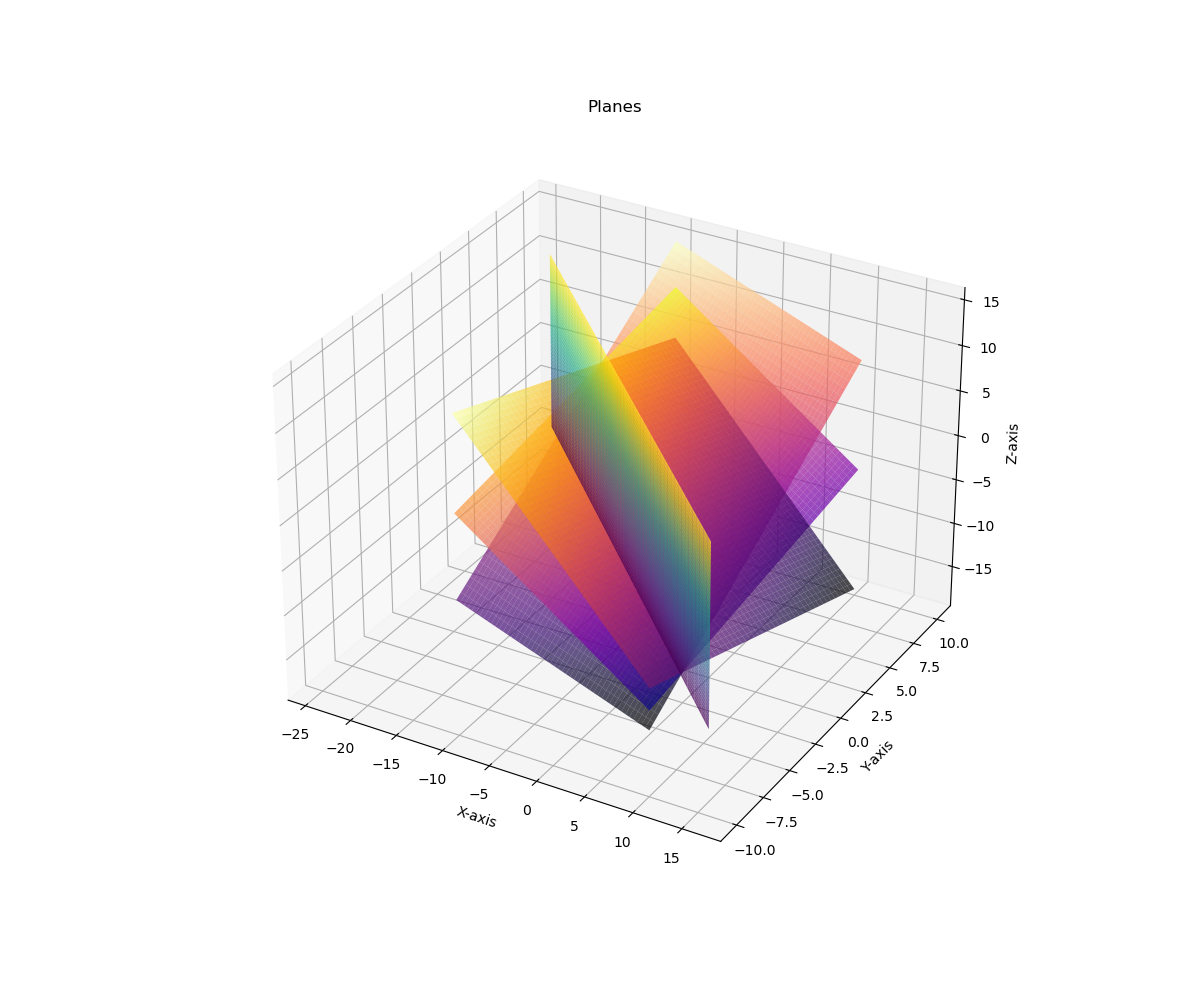
\includegraphics[width=\columnwidth, height=0.8\textheight, keepaspectratio]{figs/planes2.png}     
\end{frame}


\end{document}